\chapter{Использование направленного ответвителя на связанных линиях}

Построим модель для использования направленного ответвителя на связанных линиях как устройства ответвления мощности из основного канала в детектор мощности и влияние на него рассогласованности последнего.
Моделируемая схема представлена на Рис.~\ref{fig:afd_homework_3_schematic_1}.

\begin{figure}[!ht]
    \centering
    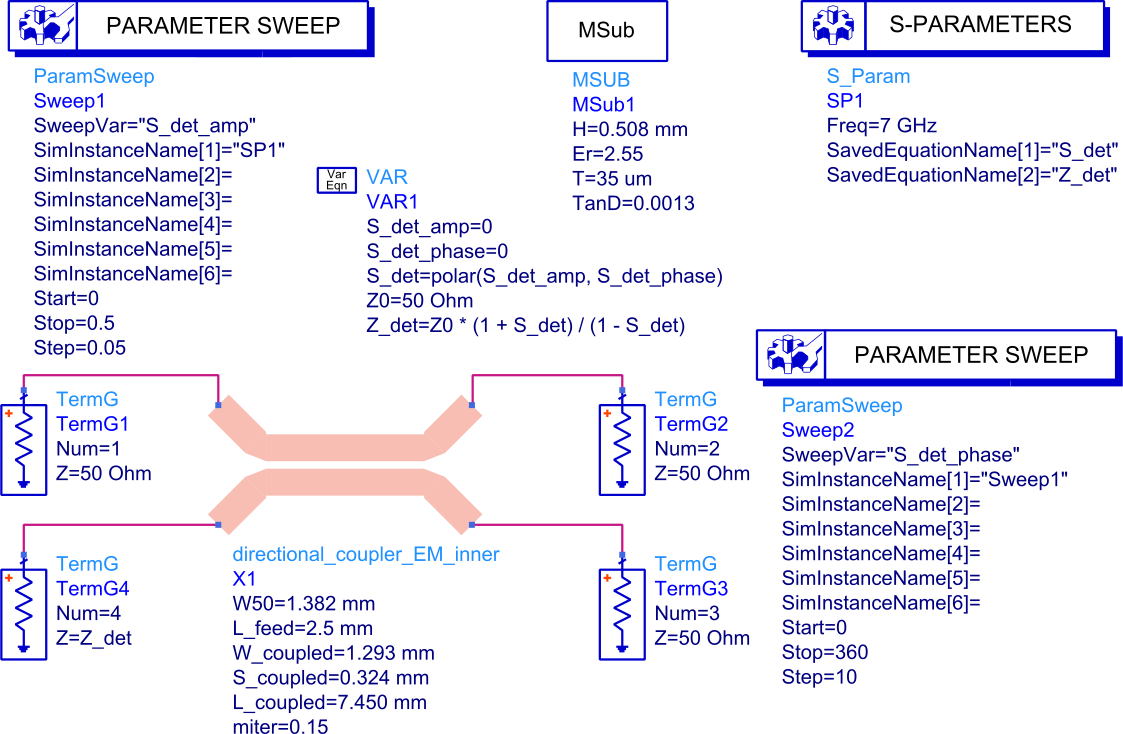
\includegraphics[width=0.7\textwidth]{afd_homework_3_schematic_1.pdf}
    \caption{Ответвитель мощности}%
    \label{fig:afd_homework_3_schematic_1}
\end{figure}

Свипать будем коэффициент отражения детектора мощности в пределах некоторого радиуса коэффициента отражения $S_\text{det\_amp}$ в отрезке [0, $0.5$].
Фазу $S_\text{det\_phase}$ прогоним во всей окружности в отрезке [0°, 360°].

$S_\text{det\_amp}$ и $S_\text{det\_phase}$ собираются в комплексный коэффициент отражения $S_\text{det}$, который в свою очередь, перечитывается в импеданс $Z_\text{det}$.
Импеданс $Z_\text{det}$ подставляется в импеданс терминатора 4, имитирующего детектор мощности.

Для использование в выражениях пробросим значения переменных $S_\text{det}$ и $Z_\text{det}$ в датасет (вкладка Output контролера симуляции SP1).

Иерархия свипов Sweep2 ($S_\text{det\_phase}$) → Sweep1 ($S_\text{det\_amp}$) → SP1 (расчет на одной частоте $7~\text{ГГц}$).

После моделирования для удобства, определим выражения вида $S_\text{xx\_dB} = S(x, x)[\dots, \dots, 0]$ (Рис.~\ref{fig:afd_homework_3_data_1_equations}) для коэффициента отражения $S_{11}$, рабочего затухания $S_{21}$, переходного ослабления $S_{41}$ и развязки $S_{31}$.
Нужно это для того, чтобы в результатах убрать зависимость от индекса частоты, равного 0.

\begin{figure}[!ht]
    \centering
    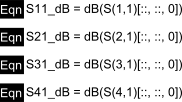
\includegraphics[width=0.4\textwidth]{afd_homework_3_data_1_equations.pdf}
    \caption{}%
    \label{fig:afd_homework_3_data_1_equations}
\end{figure}

Выведем их на прямоугольные графики для предварительного анализа (Рис.~\ref{fig:afd_homework_3_data_1_Sx1}).
Т.к. присутствует зависимость от двух независимых переменных $S_\text{det\_amp}$ и $S_\text{det\_phase}$, то отобразятся семейства графиков.

\begin{figure}[!ht]
    \centering
    \begin{subfigure}[b]{0.47\textwidth}
        \centering
        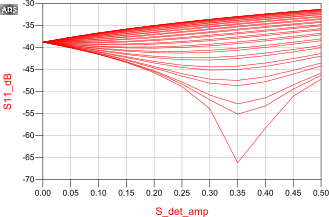
\includegraphics[width=\textwidth]{afd_homework_3_data_1_S11.pdf}
        \caption{}%
        \label{fig:afd_homework_3_data_1_S11}
    \end{subfigure}
    \hfill
    \begin{subfigure}[b]{0.47\textwidth}
        \centering
        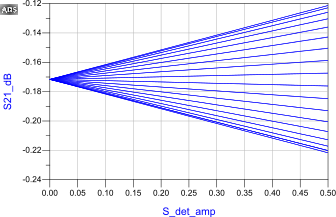
\includegraphics[width=\textwidth]{afd_homework_3_data_1_S21.pdf}
        \caption{}%
        \label{fig:afd_homework_3_data_1_S21}
    \end{subfigure}
    \vfill
    \begin{subfigure}[b]{0.47\textwidth}
        \centering
        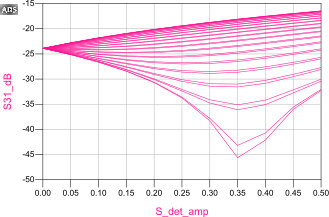
\includegraphics[width=\textwidth]{afd_homework_3_data_1_S31.pdf}
        \caption{}%
        \label{fig:afd_homework_3_data_1_S31}
    \end{subfigure}
    \hfill
    \begin{subfigure}[b]{0.47\textwidth}
        \centering
        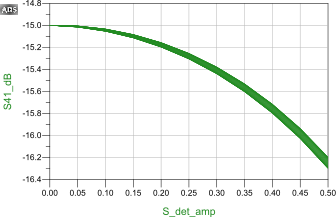
\includegraphics[width=\textwidth]{afd_homework_3_data_1_S41.pdf}
        \caption{}%
        \label{fig:afd_homework_3_data_1_S41}
    \end{subfigure}
    \caption{%
        Разброс значений элементов матрицы рассеяния:
        (а) $S_{11}$;
        (б) $S_{21}$;
        (в) $S_{31}$;
        (г) $S_{41}$
    }%
    \label{fig:afd_homework_3_data_1_Sx1}
\end{figure}

По результатам видно, что:
\begin{itemize}
    \item
        коэффициент отражения $S_{11}$ сохраняется отличным, не более $-30~\text{дБ}$;
    \item
        рабочее затухание $S_{21}$ отличное и практически не меняется;
    \item
        развязка $S_{31}$ меняется довольно сильно, но на этом выходе обычно находится согласованная нагрузка и поэтому на способность НО на связанных линиях работать как устройства подачи сигнала в детектор не влияет;
    \item
        переходное ослабление $S_{41}$ меняется от $-16.3~\text{дБ}$ до $-15~\text{дБ}$.
\end{itemize}

\begin{wrapfigure}{l}{0.5\textwidth}
    \centering
    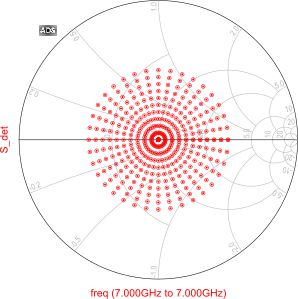
\includegraphics[width=0.5\textwidth]{afd_homework_3_data_1_smith_chart.pdf}
    \caption{}%
    \label{fig:afd_homework_3_data_1_smith_chart}
\end{wrapfigure}

Дополнительно выведем $S_\text{det}$ на отдельную диаграмму Смита, чтобы показать, при каких диапазонах $S_\text{det}$ проводилось моделирование (Рис.~\ref{fig:afd_homework_3_data_1_smith_chart}).

Переходное ослабление в применении НО на связанных линиях как устройства детектирования само по себе не всё говорит о качестве работы.
Обычно интересует значение уровня выходного сигнала с учетом рабочего затухания.
Т.е. более информативна направленность $\frac{S_{21}}{S_{41}}$, показывающая отношение выходного сигнала к ответвленному.
Поисследуем ее с помощью контуров постоянного уровня на диаграмме Смита.

Определим \code{S21toS41} на фиксированной частоте и отобразим на прямоугольном графике для предварительного анализа.

Видно, что направленность меняется в диапазоне $14.5~\text{дБ}$ до $16.1~\text{дБ}$.
Введём необходимые переменные для использования функции \code{contour\_polar}.

\begin{figure}[!ht]
    \centering
    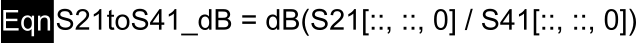
\includegraphics[width=0.5\textwidth]{afd_homework_3_data_2_equation.pdf}
    \caption{}%
    \label{fig:afd_homework_3_data_2_equation}
\end{figure}

\begin{figure}[!ht]
    \centering
    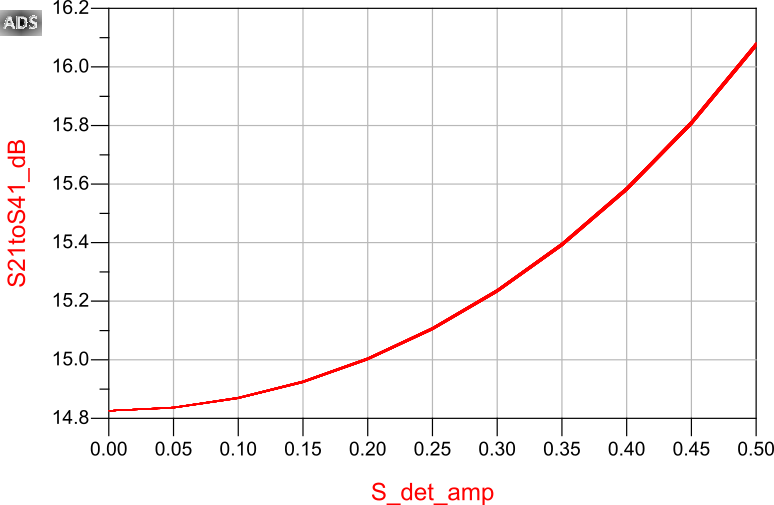
\includegraphics[width=0.7\textwidth]{afd_homework_3_data_2_response.pdf}
    \caption{}%
    \label{fig:afd_homework_3_data_2_response}
\end{figure}

Нужно задать желаемые уровни для отображения (связка \_min, \_max, \_step и \_levels).
Также задается вид интерполяции $InterpMode = 2$ (Рис.~\ref{fig:afd_homework_3_data_3_equations_1}).

\begin{figure}[!ht]
    \centering
    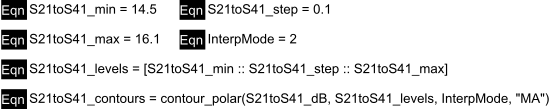
\includegraphics[width=\textwidth]{afd_homework_3_data_3_equations_1.pdf}
    \caption{}%
    \label{fig:afd_homework_3_data_3_equations_1}
\end{figure}

Отобразим на диаграмме Смита (Рис.~\ref{fig:afd_homework_3_data_3_contours_1}).

\begin{figure}[!ht]
    \centering
    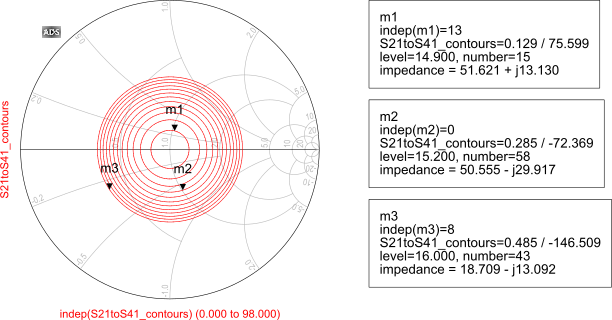
\includegraphics[width=\textwidth]{afd_homework_3_data_3_contours_1.pdf}
    \caption{}%
    \label{fig:afd_homework_3_data_3_contours_1}
\end{figure}

Видно, что до определенного уровня согласованности детектора мощности, направленность стабильна и сохраняется около $15~\text{дБ}$.
При большей рассогласованности направленность достигает $16~\text{дБ}$, что сильно отличается от целевого значения.

Добавим простую цепочку выражений, для того, чтобы определить, до какого КСВН нужно согласовать детектор мощности (Рис.~\ref{fig:afd_homework_3_data_4}).
Исходя из желаемого КСВН детектора $DetVSWR$ будет отображаться круг соответствующего коэффициента отражения $DetSin$.

\begin{wrapfigure}{r}{0.4\textwidth}
    \centering
    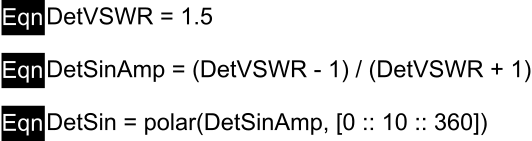
\includegraphics[width=0.4\textwidth]{afd_homework_3_data_4.pdf}
    \caption{}%
    \label{fig:afd_homework_3_data_4}
\end{wrapfigure}

Зафиксируем требование, что направленность не должна отличаться от минимальной $14.5~\text{дБ}$ более чем на $0.5~\text{дБ}$.

Т.к. уровни контуров идут от минимума к максимуму наружу, то надо найти такое максимальное значение КСВН детектора, при котором круг постоянного КСВН он не выходит за пределы контура уровня $15~\text{дБ}$.
Найденное значение КСВН детектора $1.5$ (Рис.~\ref{fig:afd_homework_3_data_5}).

\begin{figure}[!ht]
    \centering
    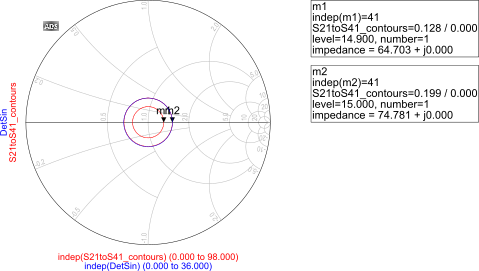
\includegraphics[width=\textwidth]{afd_homework_3_data_5.pdf}
    \caption{}%
    \label{fig:afd_homework_3_data_5}
\end{figure}

Отсюда можно сделать вывод, что на центральной частоте нужно согласовать детектор мощности на $50~\text{Ом}$ так, чтобы его КСВН не превышал $1.5$.
Тогда ошибка детектирования выходной мощности не будет превышать $0.5~\text{дБ}$.
